% B-owned results/analysis draft, generated from actual v2 artifacts on 2026-11-19.
% Compile from the repository root, or adjust the \input/\includegraphics paths.
% Requires booktabs and graphicx. Integrate the 6.2 subsection supplied by A
% between the two analysis subsections below. Citations to papers and team-wide
% numbering/bibliography must be supplied by the report integrator.
% All percentages and percentage-point differences below use exact-entity
% micro-F1; intervals are sentence-bootstrap percentile intervals unless noted.
\begingroup
\setlength{\emergencystretch}{2em}

\section{Main Results}
\label{sec:b-main-results}

\paragraph{Question and protocol.}
We ask which supervised extractor should serve as the primary system on
CoNLL-2003, and whether the method ranking persists in social-media and
restaurant-query text. We expected each step from a dictionary to learned
contextual models to improve F1, although the methods differ in more than one
component. The primary method was selected using the mean full-validation F1
of the three neural seeds, with a single run for each classical method. The
nine method--domain searches compared two \emph{joint} configurations per
model and domain using seed-0 validation, followed by three runs of the winning
neural configuration. Sentence-level bootstrap intervals below use 1,000
resamples; they measure uncertainty over sentences for a fixed trained model.
Across-seed sample standard deviations describe a different source of
variation and should not be interpreted as bootstrap confidence intervals.
% Selection/search evidence: output/b_finish_v2/frozen.json and
% output/b_tuning/selection.json. Baseline configurations are in the selected
% run_config.json files; methods are documented in B_methods_draft.tex.

\paragraph{Primary extractor and entity types.}
The validation-selected primary extractor is the fine-tuned BERT token
classifier (M4). Its three-seed mean CoNLL validation F1 is 94.278\%, compared
with 94.271\% for Span and 92.641\% for BiLSTM--CRF (M3). This very small
validation separation between M4 and Span is not evidence of a robust ranking.
For M4, the chosen CoNLL configuration uses learning rate $2\times10^{-5}$,
batch size 16, and at most three epochs, with the checkpoint chosen on
validation. On the full CoNLL test set, representative seed 0 yields precision
89.41\%, recall 91.77\%, and F1 90.57\% (95\% CI [89.67, 91.40]); its
three-seed test F1 is $90.6\pm0.2$ percentage points (sample SD). Type-level
seed-0 P/R/F1 and F1 intervals are LOC 92.76/93.71/93.23\% [92.25, 94.22],
ORG 87.16/90.73/88.91\% [87.58, 90.21], PER 95.99/94.81/95.40\%
[94.50, 96.26], and MISC 73.79/82.62/77.96\% [75.21, 80.57]. MISC is
therefore the weakest of these four reported types; that observation alone
does not explain why it is difficult.

For a complementary token-level diagnostic, the same M4 test predictions
match 45,556 of 46,435 gold BIO tags, or 98.1070\% token accuracy; 82.5304\%
of gold tokens are \texttt{O}. This is a token-weighted measure, while the
90.5723\% F1 above requires exact typed entity spans. The two quantities use
different units and denominators; their numerical difference is not a causal
attribution or a direct measure of entity errors.
% Source: output/b_finish_v2/evaluation/tasks/
% domain__M4__conll2003__conll2003__full__standard__seed0/scores.json;
% three-seed summary: output/b_finish_v2/latex_handoff/t3_b_seed_summary.tex.

\begin{table}[t]
\centering
\caption{Full native-domain supervised test results, representative seed 0.
Precision (P), recall (R), F1, and sentence-bootstrap F1 interval endpoints
are percentages. M0--M2 are A's classical methods; M3, M4, and Span are B's
neural methods.}
\label{tab:b-native-full}
% Requires booktabs and graphicx. Seed 0; exact-entity metrics in percent.
\begin{tabular}{@{}llrrrrr@{}}
\toprule
Dataset & Method & P & R & F1 & CI low & CI high \\
\midrule
CoNLL-03 & M0 & 72.1 & 46.8 & 56.7 & 55.2 & 58.1 \\
CoNLL-03 & M1 & 69.9 & 77.2 & 73.4 & 72.0 & 74.7 \\
CoNLL-03 & M2 & 82.1 & 80.8 & 81.4 & 80.2 & 82.5 \\
CoNLL-03 & M3 & 89.4 & 89.7 & 89.5 & 88.7 & 90.3 \\
CoNLL-03 & M4 & 89.4 & 91.8 & 90.6 & 89.7 & 91.4 \\
CoNLL-03 & Span & 90.1 & 90.8 & 90.4 & 89.6 & 91.3 \\
WNUT-17 & M0 & 0.0 & 0.0 & 0.0 & 0.0 & 0.0 \\
WNUT-17 & M1 & 20.1 & 11.2 & 14.4 & 12.1 & 17.1 \\
WNUT-17 & M2 & 43.1 & 9.9 & 16.1 & 13.2 & 19.3 \\
WNUT-17 & M3 & 62.1 & 11.4 & 19.3 & 15.9 & 22.8 \\
WNUT-17 & M4 & 50.4 & 35.8 & 41.8 & 38.7 & 45.3 \\
WNUT-17 & Span & 50.3 & 45.8 & 47.9 & 44.8 & 51.0 \\
MIT Rest. & M0 & 42.8 & 46.4 & 44.5 & 42.9 & 46.2 \\
MIT Rest. & M1 & 65.1 & 73.3 & 68.9 & 67.2 & 70.6 \\
MIT Rest. & M2 & 78.3 & 76.2 & 77.3 & 75.7 & 78.8 \\
MIT Rest. & M3 & 79.0 & 76.9 & 77.9 & 76.5 & 79.4 \\
MIT Rest. & M4 & 76.8 & 79.7 & 78.2 & 76.7 & 79.7 \\
MIT Rest. & Span & 79.2 & 79.9 & 79.6 & 78.2 & 81.1 \\
\bottomrule
\end{tabular}

\end{table}

\begin{table}[t]
\centering
\caption{Neural full-test F1 means and sample standard deviations across three
training seeds, in percentage points. These SDs are not sentence-bootstrap
confidence intervals.}
\label{tab:b-seed-variability}
% Neural seed variability: mean and sample SD on the same native full test.
\begin{tabular}{@{}llrr@{}}
\toprule
Dataset & Method & Mean F1 & Sample SD \\
\midrule
CoNLL-03 & M3 & 89.5 & 0.1 \\
CoNLL-03 & M4 & 90.6 & 0.2 \\
CoNLL-03 & Span & 90.3 & 0.2 \\
WNUT-17 & M3 & 23.7 & 5.0 \\
WNUT-17 & M4 & 42.3 & 1.7 \\
WNUT-17 & Span & 46.8 & 2.0 \\
MIT Rest. & M3 & 77.7 & 0.2 \\
MIT Rest. & M4 & 77.7 & 0.5 \\
MIT Rest. & Span & 79.1 & 0.7 \\
\bottomrule
\end{tabular}

\end{table}

\paragraph{Method sequence and boundary errors.}
For full CoNLL test and seed 0, F1 increases from 56.73\% (M0) to 73.39\%
(M1), 81.40\% (M2), 89.53\% (M3), and 90.57\% (M4); Span obtains 90.44\%.
The paired sentence-bootstrap differences in percentage points are
M1$-$M0 $=+16.66$ [15.13, 18.15], M2$-$M1 $=+8.01$ [7.02, 8.96],
M3$-$M2 $=+8.12$ [7.17, 9.08], M4$-$M3 $=+1.05$ [0.30, 1.81], and
Span$-$M4 $=-0.13$ [$-0.76$, 0.44]. The final interval includes zero. These
are paired comparisons of \emph{seed-0 predictions}, not uncertainty across
random initializations. Because neighboring methods change architecture,
features, optimization, and training jointly, the incremental differences do
not identify the causal contribution of any single component.

Before BIO repair, M1 produced 676 illegal inside-tag tokens across 524
CoNLL test sentences; M2 produced none. This is consistent with the sequence
constraints of the CRF, but it is not an estimate of a controlled CRF-only F1
effect. The M2 regularization parameters were originally chosen by
document-grouped five-fold cross-validation using the historical POS and chunk
features; the final baseline uses spaCy POS without chunk. We therefore do not
claim that the final feature configuration was independently re-tuned using the
same cross-validation feature set.
% BIO repair counts: output/b_finish_v2/classic/conll2003/tasks/
% conll2003__M1__full/metadata.json and conll2003__M2__full/metadata.json.
% Historical/final feature distinction: README_A.md and results/m2_cv_grid.json.

The boundary analysis pairs overlapping, non-exact spans one-to-one and
counts distinct error events. Boundary-involved events include boundary-only
and simultaneous boundary-and-type errors. They account for 163/687 (23.73\%)
of M4 events and 121/694 (17.44\%) of Span events; Span minus M4 is
$-6.29$ percentage points (paired 95\% CI [$-8.67$, $-3.99$]). The
denominator is \emph{error events}, not all entities or tokens. This supports
a seed-0 difference in error composition under this matching rule; it does not
establish that Span improves overall entity F1 or that the difference
replicates across all seeds.
% Sources: output/b_finish_v2/analysis/paired_models_conll_seed0.json and
% output/b_finish_v2/analysis/boundary_m4_span_conll_seed0.json.

\begin{figure}[t]
\centering
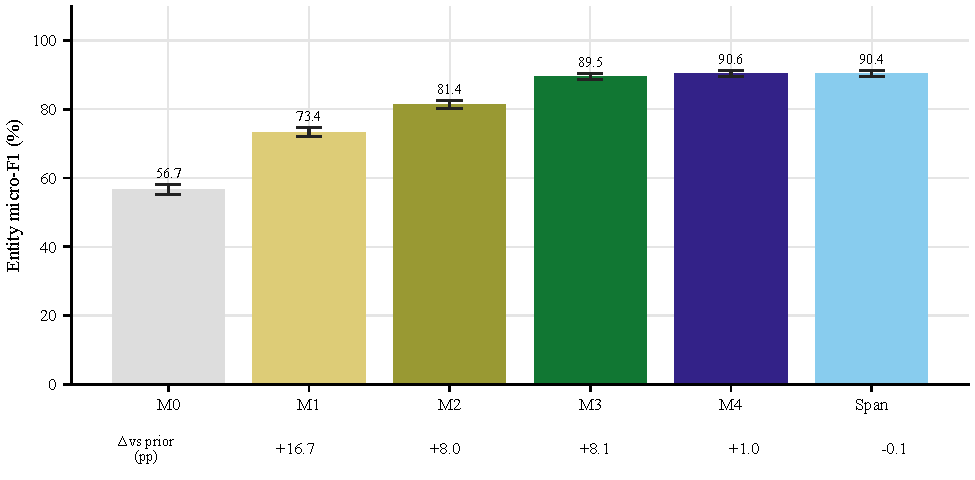
\includegraphics[width=\linewidth]{report/b/figures/f2_method_comparison.pdf}
\caption{Seed-0 full-CoNLL entity F1 with sentence-bootstrap intervals and
adjacent-method differences in percentage points. Differences are descriptive,
not isolated component effects.}
\label{fig:b-method-sequence}
\end{figure}

\paragraph{Domain ranking and matched subsets.}
On WNUT-17, the three-seed F1 means are 23.7\% for M3, 42.3\% for M4,
and 46.8\% for Span (sample SDs 5.0, 1.7, and 2.0 points, respectively).
On MIT Restaurant they are 77.7\%, 77.7\%, and 79.1\% (SDs 0.2, 0.5,
and 0.7). Thus Span has the largest observed neural mean in these two
within-domain tests, whereas M4 was selected as primary on CoNLL validation.
These results do not by themselves establish statistically significant
between-method differences for every domain. Table~\ref{tab:b-300} additionally
provides the six fixed-300 subsets and C's independently checked predictions.
Within-domain columns use their own training splits; CoNLL-trained models are
used for CoNLL++, WikiGold, and BTC. BTC uses the common PER/LOC/ORG schema,
while the other columns use their native labels, so numerical differences
between columns also reflect different annotation spaces and sample sizes.
% Tables: output/b_finish_v2/latex_handoff/t3_b_native_full.tex,
% t3_b_seed_summary.tex and t3_b_300.tex. C matching evidence:
% output/b_finish_v2/c_verified/inventory.json (24 checked points).

\begin{table}[t]
\centering
\caption{Entity F1 on the fixed 300-sentence subsets. The four lower rows are
C's previously generated predictions after checking IDs, configuration,
labels and scores against the fixed subsets. Few-shot Qwen uses ten retrieved
examples. Schemas and training sources differ across datasets; see text.}
\label{tab:b-300}
\resizebox{\linewidth}{!}{% Fixed 300 sentences per target. BTC uses PER/LOC/ORG; other columns use their native labels.
\begin{tabular}{@{}lrrrrrr@{}}
\toprule
Method & CoNLL-03 & CoNLL++ & WikiGold & BTC & WNUT-17 & MIT Rest. \\
\midrule
M0 & 60.2 & 47.0 & 24.0 & 10.8 & 0.0 & 43.6 \\
M1 & 69.9 & 65.4 & 41.4 & 26.1 & 16.7 & 67.7 \\
M2 & 81.0 & 70.3 & 57.8 & 25.2 & 20.3 & 77.8 \\
M3 & 88.5 & 82.0 & 72.5 & 31.5 & 21.0 & 77.9 \\
M4 & 88.1 & 83.9 & 79.1 & 36.6 & 45.7 & 80.3 \\
Span & 89.0 & 83.2 & 80.4 & 37.3 & 52.4 & 79.8 \\
GLiNER & 59.2 & 68.4 & 62.6 & 50.9 & 45.4 & 28.5 \\
Qwen1.5B-zero & 43.7 & 46.7 & 50.4 & 39.9 & 28.6 & 34.9 \\
Qwen7B-zero & 64.0 & 74.8 & 71.5 & 47.4 & 51.5 & 39.1 \\
Qwen7B-few & 84.5 & 81.2 & 76.3 & 55.9 & 54.8 & 71.0 \\
\bottomrule
\end{tabular}
}
\end{table}

\paragraph{Limitations of test isolation and repair.}
The repository already contained A/C held-out results before this automated
selection, so the project as a whole cannot be described as fully blinded to
test data. During v1 evaluation a tokenizer discarded the isolated U+200E
character in one BTC token. The v2 inference-only repair maps an original
token that produces no subword to the model's \texttt{[UNK]} token while
retaining the original word and output indices; models were trained before
this repair. All 162 planned tasks were rerun in a separate v2 output root.
Among the 48 completed v1 tasks that could be compared, zero showed a changed
BIO prediction at the sentence or token level; this observation does not
prove numerical determinism for other tasks. The repair was made to restore
alignment, not selected by test F1. The full audit and version comparison are
preserved in \texttt{output/b\_alignment\_audit\_v1/} and
\texttt{output/b\_finish\_v2/version\_comparison/}.
The F8 handoff contains 27 seed-level learning-curve records across three
domains and five named budgets. Training-sample IDs for 16 records match
saved ID files; for the other 11 they are only reconstructed from the shared
sampling rule, because the original selected-ID files were not saved.
Consequently, the reconstructed hashes alone cannot prove that B and C used
identical training examples. This limitation does not affect the separate
verification of the fixed test-subset IDs.
% F8 seed-level audit: output/b_finish_v2/f8_handoff/f8_b_by_seed.csv;
% handoff details: models/neural/B_HANDOFF.md.
% v2 frozen digest: cc20216cd9a430153e9d344eecb3b340bbe3ed46d559c4081ca5885300189d01.

% Insert A's 6.2 analysis between these two subsections in the combined report.
\section{Analysis}
\subsection{Where Does Supervised Performance Come From?}
\label{sec:b-representations}

\paragraph{Question, hypothesis, and method.}
We ask whether pretrained static embeddings, character information, and frozen
contextual features are associated with improved recognition when the
BiLSTM--CRF architecture and its broad training settings are held fixed. The
four representations are frozen random 100-dimensional word vectors, frozen
100-dimensional GloVe, GloVe plus a trainable character CNN, and frozen BERT
features. Static vectors are zero-padded to BERT's 768-dimensional input;
30 character dimensions are zero except in the GloVe-plus-character condition.
The random vectors are frozen and scaled to GloVe's overall standard deviation:
this is a deliberately fixed random-feature baseline, not the usual trainable
random embedding baseline. GloVe uses lowercased lookup whereas the character
CNN sees original case, so the character comparison changes case information
as well as subword representation and trainable parameters.
% Configuration and exact seeds: output/b_finish_v2/B.csv, experiment
% representation; implementation models/neural/bilstm_representations.py.

\paragraph{Results and interpretation.}
On full CoNLL test, seed-0 F1 is 59.95\% [58.39, 61.52] for frozen random
vectors, 85.65\% [84.59, 86.67] for GloVe, 89.16\% [88.23, 90.01] for
GloVe plus characters, and 90.08\% [89.20, 90.92] for frozen BERT. The
corresponding three-seed means and sample SDs are $59.59\pm0.31$,
$85.75\pm0.28$, $89.45\pm0.35$, and $89.76\pm0.28$ percentage points.
Paired sentence-bootstrap seed-0 differences are GloVe minus frozen random
$+25.70$ points [24.30, 27.07], GloVe-plus-characters minus GloVe $+3.51$
[2.71, 4.31], and frozen BERT minus GloVe-plus-characters $+0.92$ [0.22,
1.69]. The observed ordering is consistent with the hypothesis that the chosen
pretrained inputs contain useful information. The differences are not a pure
causal estimate of pretraining or capitalization: feature geometry,
vocabulary, the character encoder, and effective input information differ.
These paired intervals describe seed 0, while the reported SDs describe the
three training seeds.
% Paired results: output/b_results_analysis_v2/representations_paired_seed0.json;
% identical sentence IDs, 1,000 paired bootstrap samples, seed 42.

\begin{figure}[t]
\centering
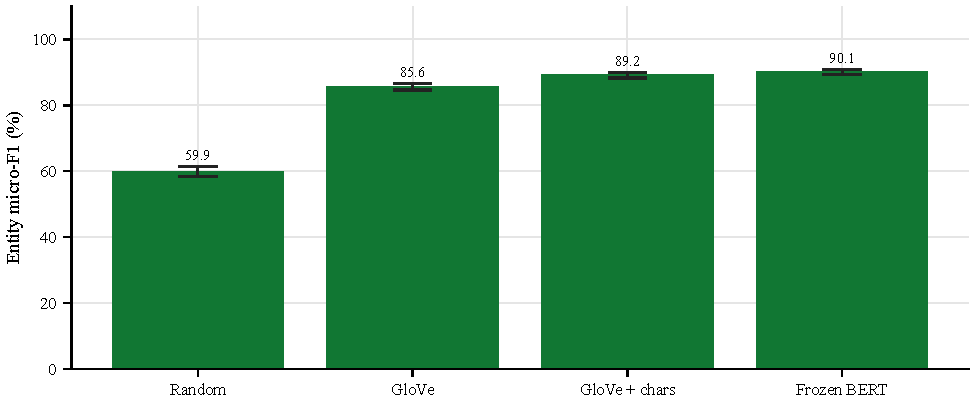
\includegraphics[width=\linewidth]{report/b/figures/f3b_bilstm_input_representations.pdf}
\caption{Input-representation comparison on the full CoNLL test set, seed 0.
Intervals are sentence-bootstrap intervals for each individual model.}
\label{fig:b-input-representations}
\end{figure}

\paragraph{Entity geometry and the MISC audit.}
For F4 we extracted gold-entity vectors on CoNLL validation, matched spans
across all three representations, and took a deterministic 1,000-span sample
from 5,840 matched spans for the plotted analysis. The K-means results on the
\emph{original} vectors (not t-SNE coordinates) are
ARI/NMI 0.223/0.219 for GloVe, 0.213/0.196 for base BERT, and 0.890/0.836
for fine-tuned BERT. The original PCA/t-SNE plotting run emitted numerical
runtime warnings. An independent single-thread OpenBLAS redraw emitted no
warnings and reproduced these ARI/NMI values; a separate recomputation also
reproduced membership for all 5,840 matched entities and all 904 MISC spans.
The checked redraw is shown below. This does not mean the two t-SNE coordinate
systems are identical: t-SNE axes have arbitrary orientation and units.
GloVe and BERT have different dimensions and pooling/coverage, and the
clustering is descriptive, not a causal test.

The separate MISC worksheet uses the \emph{full} matched validation
intersection, not the 1,000-span t-SNE sample. An assistant-prepared
preliminary review examined frequent forms and four of 12 deterministically
sampled contexts per cluster. It suggested mixed groups containing, for
example, nationality adjectives and sports-competition names; it was not an
independent human annotation or an exhaustive review. Such heterogeneity is
a plausible hypothesis about the low MISC F1, not evidence that it caused the
performance gap. \textbf{TODO (A/B):} independently review the worksheet and
merge A's feature-ablation analysis.
% Checked redraw and metadata: output/b_f4_checked_v1/manifest.json and
% output/b_f4_checked_v1/misc_cluster_audit.json; original warnings:
% output/b_finish_v2/logs/figure_f4_1.log; assisted review:
% models/neural/B_misc_cluster_review.md.

\begin{figure}[t]
\centering
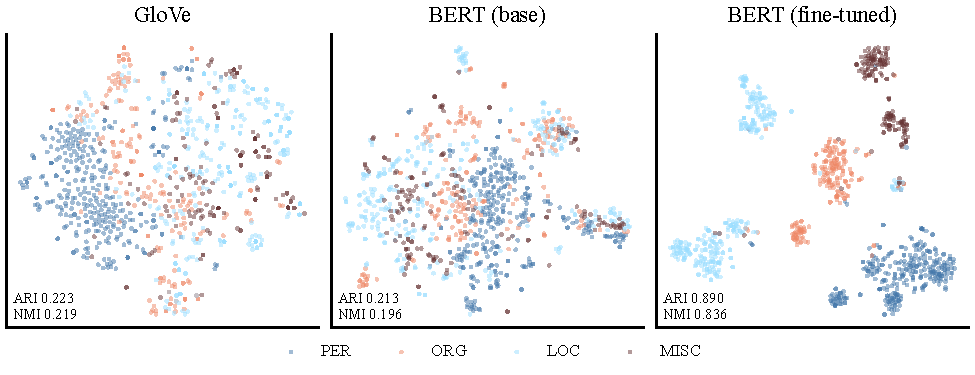
\includegraphics[width=\linewidth]{report/b/figures/f4_entity_representations_checked.pdf}
\caption{Independently redrawn F4 validation representation comparison.
The plotted set contains 1,000 matched entities; K-means metrics use the
original vectors for these same entities, rather than the t-SNE coordinates.}
\label{fig:b-entity-geometry}
\end{figure}

% A's section 6.2 should be inserted here in the final report.
\subsection{What Remains After Domain Shift?}
\label{sec:b-domain-shift}

\paragraph{Question, hypothesis, and protocol.}
We ask how a BERT model trained on news, social media, or both transfers across
five domains, and whether the observed loss is associated with entity-name
overlap or orthographic changes. The three transfer models use the shared
PER/LOC/ORG label space and seed 0. CoNLL- and WNUT-trained models inherit
their source-selected BERT configuration and native best epoch; the merged
model is selected on the combined-source validation set. Numbers in this
paragraph use full target test sets and must not be mixed with the native-label
fixed-300 results in Table~\ref{tab:b-300}.
% Sources: output/b_finish_v2/B.csv, experiment=transfer; protocol and epoch
% evidence: output/b_tuning/selection.json and output/b_finish_v2/frozen.json.

\paragraph{Transfer matrix.}
In source order CoNLL, WNUT, merged, the F1 values on CoNLL are
92.35/69.59/92.67\%; on CoNLL++ 87.73/72.41/87.85\%; and on WikiGold
79.31/64.20/79.30\%. The corresponding values are 38.30/40.12/46.85\%
on BTC and 48.01/50.69/54.95\% on WNUT. Relative to CoNLL-only training, the merged model is
8.55 points higher on BTC, 6.94 points higher on WNUT, and approximately
unchanged on WikiGold ($-0.01$ point). These are observed seed-0 differences,
not paired significance claims; training sources, example counts, and selected
checkpoints all change. Merged training does not uniformly improve every target.

\begin{figure}[t]
\centering
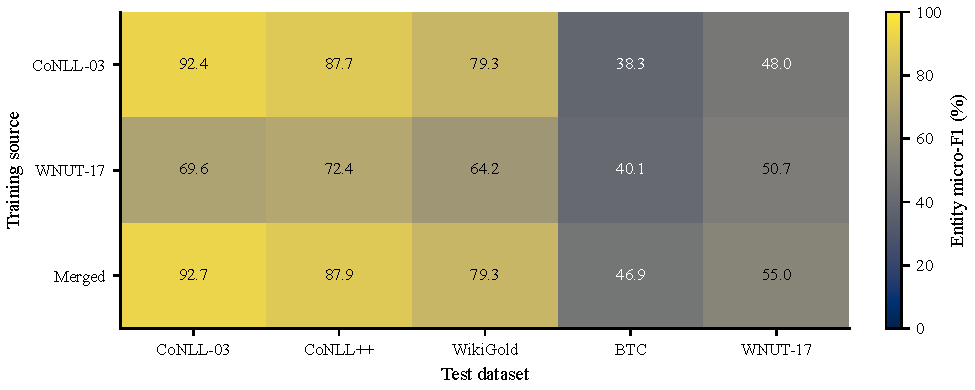
\includegraphics[width=\linewidth]{report/b/figures/f6a_bert_transfer.pdf}
\caption{Full-test BERT transfer F1 in the common three-type schema, seed 0.
Rows are the training sources and columns are targets.}
\label{fig:b-transfer}
\end{figure}

\paragraph{Name overlap and orthographic interventions.}
A's M2 overlap analysis supplies 12 CoNLL-source, non-source-domain,
entity-type points. The horizontal axis is the fraction of target gold
mentions whose full case-folded name and mapped type occur in CoNLL training;
the vertical axis is per-type M2 F1 loss relative to source-domain test F1.
The descriptive Pearson correlation is $r=-0.569$ and the fitted slope is
$-0.482$ loss percentage points per overlap percentage point. These are
\emph{M2}, not BERT, results; points share datasets and types, so neither the
correlation nor the regression establishes an independent causal relationship.
% output/b_finish_v2/analysis/f6b_from_a_m2.json; underlying analysis by A:
% results/m2_transfer_overlap.json.

\begin{figure}[t]
\centering
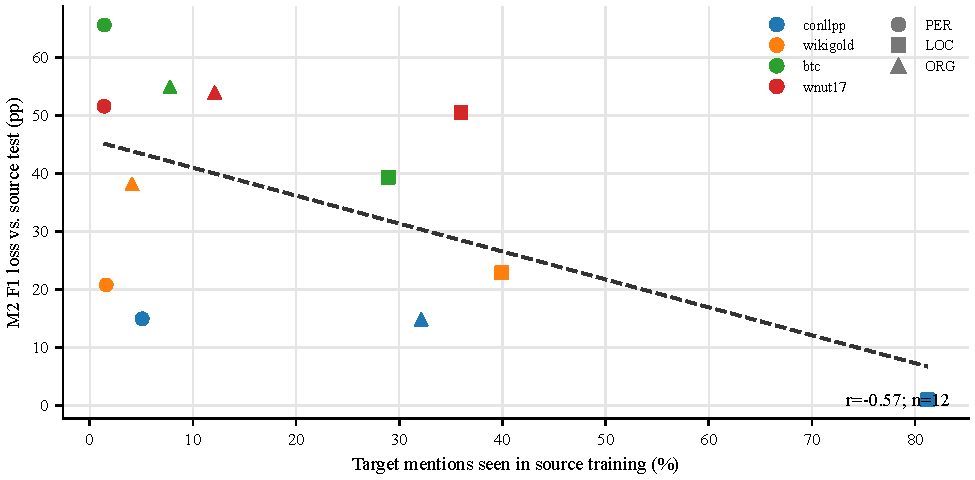
\includegraphics[width=\linewidth]{report/b/figures/f6b_crf_overlap_from_a.pdf}
\caption{A's M2 entity-overlap analysis for a CoNLL training source. Points
represent target-domain/entity-type combinations; the fitted line describes
an association rather than a causal effect.}
\label{fig:b-transfer-overlap}
\end{figure}

For M4 on 3,453 paired CoNLL test sentences, lowercasing changes F1 from
90.57\% to 30.74\%, a difference of $-59.83$ points (paired 95\% CI
[$-61.64$, $-57.99$]); 5\% character-level spelling noise changes it to
81.37\% ($-9.20$ [$-10.03$, $-8.38$]), and punctuation removal to 83.08\%
($-7.50$ [$-8.65$, $-6.49$]). On the separately constructed 500-sentence
entity-replacement pairs, F1 changes from 95.02\% to 92.65\%, a difference of
$-2.37$ points [$-3.37$, $-1.30$]. Each interval resamples the same sentence
pairs, and the replacement comparison uses its own original and modified gold
labels. These controlled transformations demonstrate sensitivity of this
trained model to the specified changes, but lowercasing alters token forms
throughout the sentence and is not a clean estimate of capitalization alone.
It also cannot be directly subtracted from the BTC transfer loss: corpus,
label space, and many linguistic properties change simultaneously. A's CRF
feature ablations and C's perturbation interpretations remain to be integrated.
% Sources: output/b_finish_v2/additional_analysis/paired__M4__*.json;
% perturbations and replacement are generated by A's documented data pipeline.
\endgroup
